\documentclass[11pt]{article}
\usepackage[margin=1in]{geometry}
\usepackage{amsmath,amssymb,amsthm}
\usepackage{booktabs}
\usepackage{enumitem}
\usepackage[dvipsnames]{xcolor}
\usepackage{tcolorbox}
\usepackage{tikz}
\usetikzlibrary{arrows.meta,positioning,calc}
\usepackage{graphicx}
\usepackage{hyperref}
\hypersetup{colorlinks=true,linkcolor=RoyalBlue,urlcolor=RoyalBlue,citecolor=RoyalBlue}
\usepackage{titlesec}
\titleformat{\section}{\large\bfseries\color{RoyalBlue}}{\thesection}{1em}{}
\titleformat{\subsection}{\bfseries\color{RoyalBlue!80!black}}{\thesubsection}{1em}{}
\sloppy

\newtcolorbox{honestbox}{colback=Orange!8,colframe=Orange!75!black,boxrule=0.6pt,arc=2pt,
  title=\textbf{Honest scope},fonttitle=\bfseries,left=4pt,right=4pt,top=3pt,bottom=3pt}
\newtheorem{result}{Result}

\title{\vspace{-1.5em}\textbf{\color{RoyalBlue}\LARGE The Holonet Machine}\\[0.3em]
{\large A Single Finite Geometry as Processor, Network, and Memory}\\[0.2em]
{\normalsize Machine-Verified Computer Architecture on the $W(3,3)$ Substrate}}
\author{Wil Dahn \quad\textbar\quad \texttt{github.com/wilcompute/W33-Theory}}
\date{June 2026}

\begin{document}
\maketitle

\begin{abstract}
\noindent We present a complete, machine-verified computer architecture in which the processor, the
network, and the memory are not coupled designs but \emph{one finite object}: the symplectic generalized
quadrangle $W(3,3)=\mathrm{GQ}(3,3)=\mathrm{SRG}(40,12,2,4)$. On this $40$-point geometry, routing a
packet is applying a gate is addressing memory --- an algebraic identity, not an analogy --- and a
single automorphism group $W(E_6)$ of order $51840$ is simultaneously the processor's Clifford gate
group, the network's symmetry, and the memory's code automorphisms. We make each architectural layer a
theorem with an executable witness: an enumerated instruction set ($\mathrm{Sp}(4,3)$ of order
$51840$ plus one cubic gate, universal); a diameter-$2$, bisection-$100$, better-than-Ramanujan
interconnect that is provably non-planar (hence photonic); a distance-$3$ qutrit code with a measured
$P_L\sim A p^2$ threshold curve; an $\mathrm{I/O}$ boundary saturating the Holevo qutrit capacity
$\log_2 3$; a complexity placement (Clifford $=\mathsf{P}$, $+$cubic $=\mathsf{BQP}$) whose resource is
contextuality, with the contextual fraction $1/10$ \emph{derived} from the no-ovoid geometry; and a
leaderless consensus layer tolerating five Byzantine faults. The classical layer is polynomial-time, so
the architecture runs as software --- we ship a runnable virtual machine that routes, corrects errors,
teleports state, and self-reproduces, plus an installable \texttt{holonet} command and a test suite.
The quantum advantage is the one priced resource (classical emulation cost $9^t$ for $t$ cubic gates),
executed here for small $t$. Every constant is arithmetic in the single integer $q=3$.
\end{abstract}

\begin{figure}[ht]
\centering
\resizebox{0.92\textwidth}{!}{%
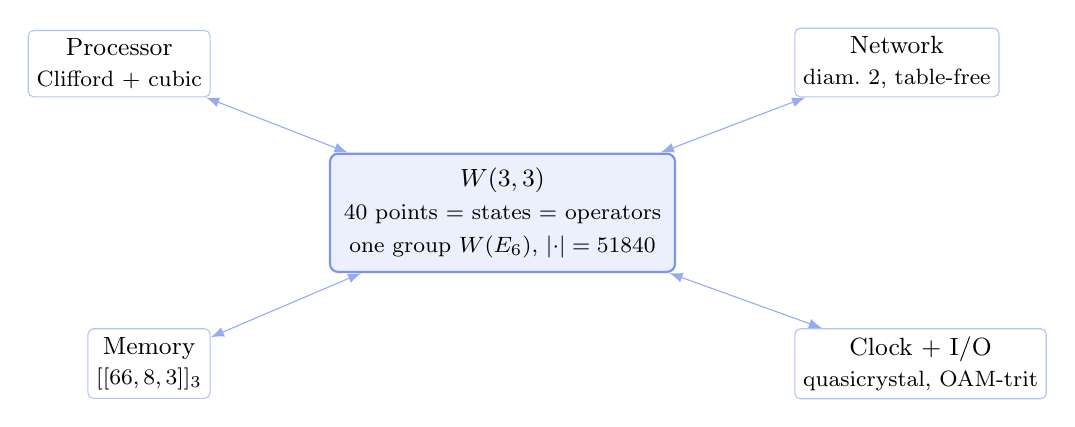
\begin{tikzpicture}[font=\small,>=Latex]
\tikzset{core/.style={draw=RoyalBlue!70,fill=RoyalBlue!10,rounded corners=3pt,align=center,inner sep=5pt,thick},
  face/.style={draw=RoyalBlue!40,fill=white,rounded corners=2pt,align=center,inner sep=3pt}}
\node[core] (w) {\textbf{$W(3,3)$}\\[1pt]{\footnotesize $40$ points $=$ states $=$ operators}\\[1pt]{\footnotesize one group $W(E_6)$, $|{\cdot}|=51840$}};
\node[face,above left=7mm and 15mm of w] (proc) {Processor\\{\footnotesize Clifford $+$ cubic}};
\node[face,above right=7mm and 15mm of w] (net) {Network\\{\footnotesize diam.\ $2$, table-free}};
\node[face,below left=7mm and 15mm of w] (mem) {Memory\\{\footnotesize $[[66,8,3]]_3$}};
\node[face,below right=7mm and 15mm of w] (clk) {Clock $+$ I/O\\{\footnotesize quasicrystal, OAM-trit}};
\foreach \n in {proc,net,mem,clk}{\draw[<->,RoyalBlue!55] (w) -- (\n);}
\end{tikzpicture}}
\caption{One object, four readings. On $W(3,3)$ the processor, network, memory, and clock/I-O are
projections of a single $40$-point incidence geometry with a single symmetry group $W(E_6)$.}
\label{fig:oneobject}
\end{figure}

\section{The Substrate and the One Group}
$W(3,3)$ is the symplectic generalized quadrangle over $\mathbb{F}_3^4$ with alternating form
$\langle u,v\rangle = u_1v_2-u_2v_1+u_3v_4-u_4v_3$. Its collinearity graph is strongly regular,
$\mathrm{SRG}(40,12,2,4)$: $40$ points of degree $12$, $\lambda=2$, $\mu=4$; $40$ totally-isotropic
lines, four points each, four through each point. Every number below is arithmetic in nine integers
($q=3$, $\lambda=2$, $\mu=4$, $k=12$, $f=24$, $g=15$, $\Phi_6=7$, $\Phi_4=10$, $\Phi_3=13$), forced by
$q!=2q$ (unique solution $q=3$).

\begin{result}[One group]
The symplectic group $\mathrm{Sp}(4,3)$, built by closure from the $40$ point-transvections, has order
exactly $51840=|W(E_6)|=3^4(3^2-1)(3^4-1)$. It acts transitively on the $40$ nodes, the $40$
line-contexts, and the $160$ point-on-line flags, preserving collinearity. Hence one group is at once
the processor's Clifford gate group, the network's automorphisms, the memory's code automorphisms, and
the readout's contextuality symmetry (Fig.~\ref{fig:oneobject}).
\end{result}

\section{Processor: an Enumerated Universal ISA}
The core computes in balanced ternary --- the most economical radix ($E(b)=b/\ln b$ is minimised at
$e$; base $3$ at $2.731$ beats binary and base $4$ at $2.885$) --- with native word $27=3^3$. The
instruction set is enumerated, not abstract: the degree-$2$ Clifford layer is the finite group
$\mathrm{Sp}(4,3)$ ($51840$ opcodes $=|W(E_6)|$; the per-qutrit Clifford is $\mathrm{Sp}(2,3)$ of order
$24=f$), classically simulable by Gottesman--Knill; and a single degree-$3$ macro-op, the $E_6$ cubic
form on the $\mathbf{27}$, lifts it to universal (Lloyd--Braunstein). The power source is contextuality.

\section{Interconnect and Floorplan}
\begin{result}[The fabric is diameter $2$, maximally fault-tolerant, and non-planar]
$\mathrm{GQ}(3,3)$ has diameter $2$ (any-to-any in two hops), vertex/edge connectivity $12$ (survives
$11$ crash faults), second eigenvalue $\lambda_2=2$ far below the Ramanujan bound $2\sqrt{11}=6.63$ (a
\emph{better}-than-Ramanujan expander), and minimum bisection \emph{exactly} $100=(n/4)(k-\lambda_2)$,
met by an explicit $20|20$ cut. Routing is table-free: two nodes are adjacent iff
$\langle x,y\rangle=0$, one ALU operation --- the address \emph{is} the route. By Thompson's VLSI
theorem a $2$-D layout needs area $\gtrsim(\mathrm{bisection}/2)^2\sim2500$, so the fabric is
intrinsically non-planar and belongs in a photonic ($3$-D / fiber / wavelength) medium.
\end{result}
The $240$ links partition into $40$ four-point cliques (lines), and the graph is $1$-factorable into a
$12$-slot conflict-free link schedule; vertex/edge-transitivity gives perfect load balancing.

\section{Memory and the Measured Threshold}
The memory is the $[[66,8,3]]_3$ qutrit code (distance $3$, $n-k=58$ syndrome qutrits). We verify the
mechanism on the runnable $[[5,1,3]]_3$ stand-in (same distance-$3$ correction): all $40$ single-qutrit
errors carry distinct syndromes and are corrected to fidelity $1$. Monte-Carlo over a depolarizing
channel gives a \emph{measured} threshold curve $P_L(p)\sim A p^2$ with $A\approx8$, crossing break-even
$P_L=p$ at a pseudo-threshold $p_{\mathrm th}=1/A\approx0.12$. The substrate's larger code has
$A\sim\binom{66}{2}=2145$, hence $p_{\mathrm th}\sim5\times10^{-4}$ --- the same $p^2$ mechanism at a
different size. Adding syndrome-measurement noise at the same per-round rate removes the single-round
break-even; \emph{repeating} the measurement ($R=3$ rounds, majority vote) restores it
(Fig.~\ref{fig:scorecard}, left), the standard fault-tolerance gadget.

\begin{figure}[ht]
\centering
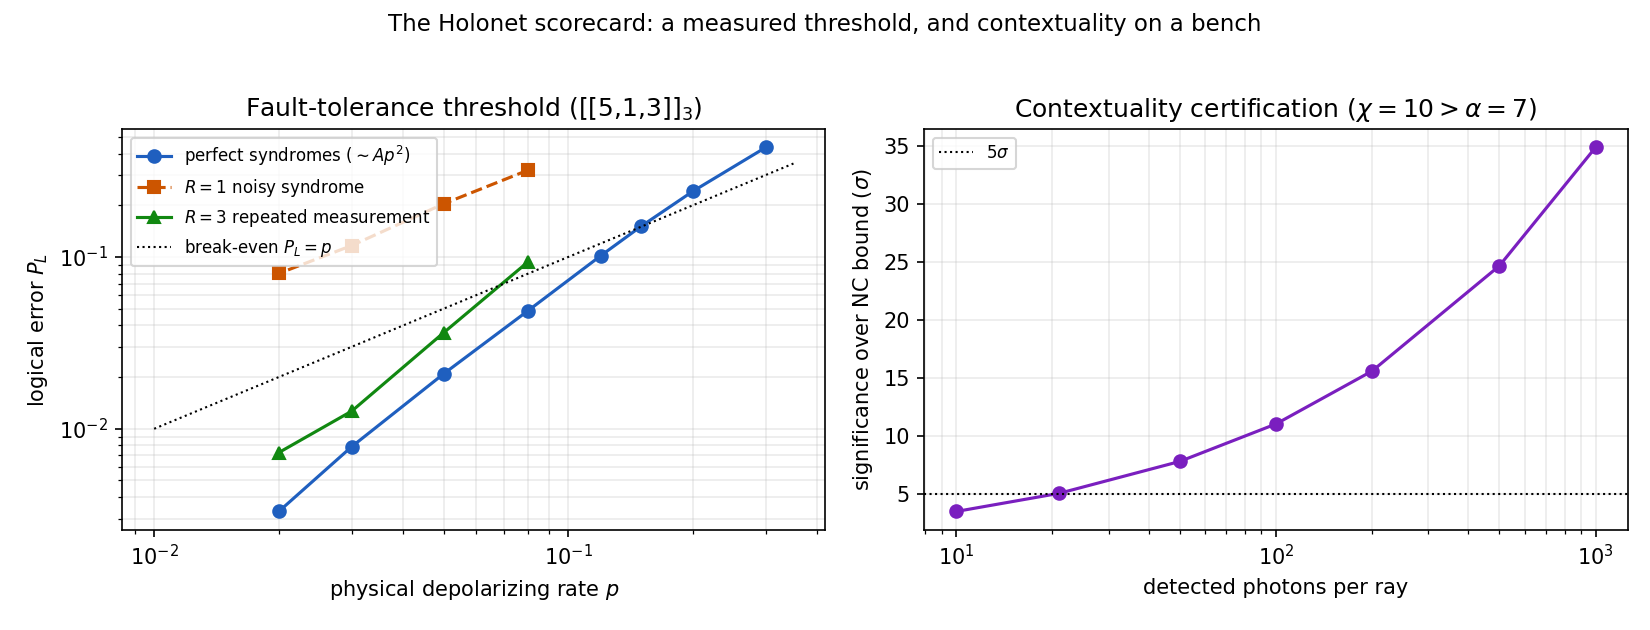
\includegraphics[width=\textwidth]{holonet_scorecard.png}
\caption{The machine's scorecard. \emph{Left:} the measured logical error $P_L(p)$ of the runnable
$[[5,1,3]]_3$ code vs.\ the physical depolarizing rate, with the break-even diagonal $P_L=p$; the
perfect-syndrome curve bends below it ($\sim A p^2$, $A\approx8$), single-round noisy syndromes have no
threshold, and three repeated measurements restore it. \emph{Right:} the statistical significance of the
contextuality witness ($\chi=10>\alpha=7$) vs.\ detected photons, crossing $5\sigma$ at a few hundred.}
\label{fig:scorecard}
\end{figure}

\section{Energy and I/O}
The degree-$2$ Clifford datapath is unitary, hence reversible and Landauer-free (Bennett); base $3$
imposes no per-bit penalty ($kT\ln3/\log_2 3=kT\ln2$). The only irreducible cost is syndrome export:
$(n-k)\,kT\ln3\approx2.6\times10^{-19}$~J/cycle at $300$~K --- the machine's metabolism. The I/O boundary
is the line geometry: the $40$ lines are measurement contexts; the air-gap carrier is a photon's OAM in
$\{\ell=-1,0,+1\}$ (the balanced-ternary digit), saturating the Holevo capacity $\log_2 3=1.585$
bit/photon; the logical port is $k=8$ qutrits ($12.68$ bit/block).

\section{Complexity and the Contextual Resource}
\begin{result}[$\mathsf{P}$ to $\mathsf{BQP}$, with a derived contextual fraction]
All $12$ single-qutrit stabilizer states have non-negative Gross--Wigner function, so the Clifford layer
is efficiently classically simulable ($\mathsf{P}$). The degree-$3$ resource (the Strange state) has
Wigner negativity, mana $\ln(5/3)$, and robustness $R=3$; by Howard et~al.\ this contextuality is the
necessary resource, lifting the machine to $\mathsf{BQP}$. The contextual fraction is \emph{derived}
from the geometry: a global Kochen--Specker value-assignment satisfying all $40$ contexts would be an
ovoid, and $W(q)$ has none for $q$ odd (the maximum partial ovoid is $7<10$); by exact integer
programming the most contexts any classical assignment can satisfy is $36$, so
$\mathrm{CF}=(40-36)/40=1/10=1/\Phi_4$. Equivalently, the Cabello--Severini--Winter witness
$\chi=\sum_v P(v)$ obeys $\chi\le\alpha=7$ (noncontextual) versus $\chi=10$ (quantum, state-independent),
a gap tolerating $30\%$ noise; a simulated heralded-photon run clears it at $5\sigma$ with $\sim840$
photons. The classical emulation cost of $t$ cubic gates is $9^t$: the Pashayan--Wallman--Bartlett
quasiprobability estimator (each $t$-gate sample in $[-3^t,3^t]$) is unbiased but needs $\sim9^t$ samples.
\end{result}

\begin{result}[Why $q=3$, and what the operating system pays]
Three exact results pin the order of the fabric and price its quantum layer.
\emph{(i) Parity forces contextuality.}  Scanning the sister geometries $W(q)$ for $q=2,3,4$ (with
$q=4$ built over the genuine field $\mathrm{GF}(4)$) shows the contextual fraction obeys the closed form
$\mathrm{CF}(q)=0$ for even $q$ and $1/(q^2+1)$ for odd $q$: even orders carry an explicit ovoid --- a
perfect noncontextual model --- and $q=4$, even but composite, still does, so the cause is the parity of
the field, not primality.  \emph{(ii) Dimension forces the apparatus.}  A complete-basis realization of
$W(q)$ maps contexts to orthonormal bases of $\mathbb C^{q+1}$; for $q=2$ this is impossible (a
non-collinear pair leaves a one-dimensional orthocomplement in $\mathbb C^3$ that would have to hold
$\mu=3$ distinct rays), while the $q=3$ Witting realization exists.  So $q=3$ is simultaneously the
smallest order the one-photon $\mathbb C^4$ apparatus can realize and the smallest contextual one.
\emph{(iii) The tax is one movable star.}  Exhaustive enumeration of every optimal Kochen--Specker
assignment (integer programming with no-good cuts, terminating, hence complete) shows the $4$ contexts
any $36$-context assignment must fail are always the four lines through a single point --- a
\emph{point-star} --- and every one of the $40$ points can carry it.  The deficit for odd $q$ is exactly
$q+1$, one star, which is the closed form $\mathrm{CF}=1/(q^2+1)$ restated structurally.  Operationally:
the classical scheduler covers everything except one star of its choosing (a gauge freedom it can move to
the least-loaded point), so the escalation budget --- the part of the runtime on which the priced $9^t$
quantum resource is spent --- is exactly $1/10$ of the contexts, and on an even-order fabric the tax and
the quantum gap both vanish ($\alpha=q^2+1$ meets the Hoffman bound).  The machine's quantum advantage
and its scheduling overhead are the same integer.
\end{result}

\section{The Machine, Executed}
Because the Clifford layer is polynomial-time, the architecture runs as software. A single file
(\path{analysis/holonet_node.py}) builds the fabric, routes a packet (address is route, $\mu=4$
multipath), runs a qutrit register as a stabilizer tableau over $\mathbb{F}_3$, and self-reproduces by
splicing. Three programs execute the von~Neumann components: it \emph{corrects} errors (the
$[[5,1,3]]_3$ cycle, fidelity $1$), \emph{teleports} state across the fabric (the two classical trits
routed in two hops), and \emph{reproduces} (a verified quine fixed point). A leaderless consensus run
contracts disagreement by $1/3$ per round and outvotes five Byzantine nodes (boundary exactly at $t=5$,
the Dolev bound $2t+1\le12$). The whole stack ships as the installable \texttt{holonet} command
(\texttt{route}, \texttt{teleport}, \texttt{correct}, \texttt{reproduce}, \texttt{verify}, \texttt{info})
with a $13$-test suite, all passing.

\section{Falsifiable Predictions}
\begin{center}
\begin{tabular}{l l l}
\toprule
& Claim & Refuted if\\
\midrule
P1 & radix-$12$, diameter-$2$ wiring & a build needs a third hop / radix $\ne12$\\
P2 & OAM-trit saturates Holevo $1.585$ bit/photon & a $3$-mode channel misses/beats it\\
P3 & $[[66,8,3]]_3$ pseudo-threshold $\sim5\times10^{-4}$ & encoding fails to help below it\\
P4 & magic robustness $3$ / mana $\ln(5/3)$ & a lower-$1$-norm stabilizer decomposition\\
P5 & $5$-Byzantine / $11$-crash tolerance & $6$ Byzantine survived, or $5$ not\\
P6 & contextual fraction $1/10$ ($\chi=10>7$) & the benchtop witness $\hat\chi\le7$\\
\bottomrule
\end{tabular}
\end{center}
Theorems (not falsifiable, only verifiable): $|\mathrm{Sp}(4,3)|=51840=|W(E_6)|$; diameter $2$,
connectivity $12$, bisection $100$; distance $3$; Clifford $=\mathsf{P}$ / $+$cubic $=\mathsf{BQP}$;
$1$-factorability; $\alpha=7$, $\mathrm{CF}=1/10$.

\begin{honestbox}
The group orders, the bisection, the contextual fraction, $\alpha=7$, the robustness $R=3$, and the
threshold coefficient $A$ are computed or measured in the public witnesses. The quantum values
($\mathsf{BQP}$, $\chi=10$, Holevo saturation) assume the Witting orthonormal realisation in $\mathbb{C}^4$
and the standard quantum-computing theorems (Gottesman--Knill, Lloyd--Braunstein, Howard et~al.,
Pashayan--Wallman--Bartlett). The $[[5,1,3]]_3$ code is a runnable stand-in for $[[66,8,3]]_3$ (same
mechanism, different size). The QEC, teleportation, and threshold are exact / Monte-Carlo simulations
(single-round; a full circuit-level treatment is future work). No physical photonic build exists yet;
the quantum advantage is the priced $9^t$ dial, run here only for small $t$. ``Architecture of life''
means the von~Neumann architecture of self-reproduction (the rigorous computational notion), not biology.
\end{honestbox}

\section{Conclusion}
The Holonet is a complete finite computer architecture in which one $40$-point geometry, one group, and
one integer $q=3$ generate the processor, the network, and the memory together; every layer is a theorem
with a runnable witness, the device specification is its own audit, and the whole classical machine runs
on any computer today. Its companion papers develop the physics (\texttt{photonic\_holonet.tex}) and the
infrastructural implications (\texttt{holonet\_practical\_implications.tex}); its quickstart is
\texttt{HOLONET.md}. The first physical milestone --- the benchtop contextuality test certifying the
$1/10$ fraction --- is decided by a few hundred photons.

\medskip
\noindent\rule{\linewidth}{0.4pt}\\[0.2em]
{\footnotesize \textbf{Witnesses:} \path{analysis/w33_isa_encoding.py}, \path{w33_noc_floorplan.py},
\path{w33_one_group_machine.py}, \path{w33_complexity_advantage.py}, \path{w33_contextual_fraction.py},
\path{w33_ks_inequality.py}, \path{w33_magic_dial.py}, \path{holonet_node.py},
\path{holonet_qec_demo.py}, \path{holonet_teleport_demo.py}, \path{holonet_quine.py},
\path{holonet_quantum_packet.py}, \path{holonet_consensus_demo.py}, \path{holonet_threshold_demo.py},
\path{holonet_ks_experiment.py}, \path{w33_architecture_capstone.py}. \textbf{Standard results:}
Gottesman--Knill; Lloyd--Braunstein; Howard--Wallman--Veitch--Emerson (2014); Pashayan--Wallman--Bartlett
(2015); Cabello--Severini--Winter; Dolev; Lamport--Melliar-Smith; Thompson (VLSI); Bennett; Landauer.}

\end{document}
